\documentclass[review]{elsarticle}

\usepackage{multirow}
\usepackage{lineno}
\usepackage{xspace}
\usepackage{threeparttable}
\usepackage{subfig}
\modulolinenumbers[5]

\journal{Progress in Nuclear Energy}

%% `Elsevier LaTeX' style
\bibliographystyle{elsarticle-num}
%%%%%%%%%%%%%%%%%%%%%%%

%%%% packages and definitions (optional)
\usepackage{placeins}
\usepackage{booktabs} % nice rules (thick lines) for tables
\usepackage{microtype} % improves typography for PDF
\usepackage{hhline}
\usepackage{amsmath}
\usepackage{subfig}

%\usepackage[demo]{graphicx}
%\usepackage{caption}
%\usepackage{subcaption}

\usepackage{booktabs}
\usepackage{threeparttable, tablefootnote}

\usepackage{tabularx}
\newcolumntype{b}{>{\hsize=1.0\hsize}X}
\newcolumntype{s}{>{\hsize=.5\hsize}X}
\newcolumntype{m}{>{\hsize=.75\hsize}X}
\newcolumntype{x}{>{\hsize=.25\hsize}X}

\newcommand{\Cyclus}{\textsc{Cyclus}\xspace}%
\newcommand{\Cycamore}{\textsc{Cycamore}\xspace}%
\graphicspath{ {images/} }

% tikz %
\usepackage{tikz}
\usetikzlibrary{positioning, arrows, decorations, shapes}

\usetikzlibrary{shapes.geometric,arrows}
\tikzstyle{process} = [rectangle, rounded corners, minimum width=3cm, minimum height=1cm,text centered, draw=black, fill=blue!30]
\tikzstyle{object} = [ellipse, rounded corners, minimum width=3cm, minimum height=1cm,text centered, draw=black, fill=green!30]
\tikzstyle{arrow} = [thick,->,>=stealth]

% hyperref %
\usepackage[hidelinks]{hyperref}
% after hyperref %
\usepackage{cleveref}
\usepackage{datatool}
\usepackage[acronym,toc]{glossaries}
%\newacronym{<++>}{<++>}{<++>}
\newacronym[longplural={metric tons of heavy metal}]{MTHM}{MTHM}{metric ton of heavy metal}
\newacronym{ABM}{ABM}{agent-based modeling}
\newacronym{ACDIS}{ACDIS}{Program in Arms Control \& Domestic and International Security}
\newacronym{ADS}{ADS}{Accelerator-Driven System}
\newacronym{AFCI}{AFCI}{Advanced Fuel Cycles Initiative}
\newacronym{AHTR}{AHTR}{Advanced High Temperature Reactor}
\newacronym{ANDRA}{ANDRA}{Agence Nationale pour la gestion des D\'echets RAdioactifs, the French National Agency for Radioactive Waste Management}
\newacronym{ANL}{ANL}{Argonne National Laboratory}
\newacronym{ANS}{ANS}{American Nuclear Society}
\newacronym{API}{API}{application programming interface}
\newacronym{ARE}{ARE}{Aircraft Reactor Experiment}
\newacronym{ARFC}{ARFC}{Advanced Reactors and Fuel Cycles}
\newacronym{ASME}{ASME}{American Society of Mechanical Engineers}
\newacronym{ASTRID}{ASTRID}{Advanced Sodium Technological Reactor for Industrial Demonstration}
\newacronym{ATWS}{ATWS}{Anticipated Transient Without Scram}
\newacronym{BDBE}{BDBE}{Beyond Design Basis Event}
\newacronym{BIDS}{BIDS}{Berkeley Institute for Data Science}
\newacronym{BWR}{BWR}{Boiling Water Reactor}
\newacronym{CAFCA}{CAFCA}{ Code for Advanced Fuel Cycles Assessment }
\newacronym{CDTN}{CDTN}{Centro de Desenvolvimento da Tecnologia Nuclear}
\newacronym{CEA}{CEA}{Commissariat \`a l'\'Energie Atomique et aux \'Energies Alternatives}
\newacronym{CI}{CI}{continuous integration}
\newacronym{CNEN}{CNEN}{Comiss\~{a}o Nacional de Energia Nuclear}
\newacronym{CNERG}{CNERG}{Computational Nuclear Engineering Research Group}
\newacronym{COSI}{COSI}{Commelini-Sicard}
\newacronym{COTS}{COTS}{commercial, off-the-shelf}
\newacronym{CSNF}{CSNF}{commercial spent nuclear fuel}
\newacronym{CTAH}{CTAHs}{Coiled Tube Air Heaters}
\newacronym{CUBIT}{CUBIT}{CUBIT Geometry and Mesh Generation Toolkit}
\newacronym{CURIE}{CURIE}{Centralized Used Fuel Resource for Information Exchange}
\newacronym{DAG}{DAG}{directed acyclic graph}
\newacronym{DANESS}{DANESS}{Dynamic Analysis of Nuclear Energy System Strategies}
\newacronym{DBE}{DBE}{Design Basis Event}
\newacronym{DESAE}{DESAE}{Dynamic Analysis of Nuclear Energy Systems Strategies}
\newacronym{DHS}{DHS}{Department of Homeland Security}
\newacronym{DOE}{DOE}{Department of Energy}
\newacronym{DRACS}{DRACS}{Direct Reactor Auxiliary Cooling System}
\newacronym{DRE}{DRE}{dynamic resource exchange}
\newacronym{DSNF}{DSNF}{DOE spent nuclear fuel}
\newacronym{DYMOND}{DYMOND}{Dynamic Model of Nuclear Development }
\newacronym{EBS}{EBS}{Engineered Barrier System}
\newacronym{EDF}{EDF}{Électricité de France}
\newacronym{EDZ}{EDZ}{Excavation Disturbed Zone}
\newacronym{EIA}{EIA}{U.S. Energy Information Administration}
\newacronym{EPA}{EPA}{Environmental Protection Agency}
\newacronym{EPR}{EPR}{European Pressurized Reactor}
\newacronym{EP}{EP}{Engineering Physics}
\newacronym{EU}{EU}{European Union}
\newacronym{FCO}{FCO}{Fuel Cycle Options}
\newacronym{FCT}{FCT}{Fuel Cycle Technology}
\newacronym{FEHM}{FEHM}{Finite Element Heat and Mass Transfer}
\newacronym{FEPs}{FEPs}{Features, Events, and Processes}
\newacronym{FHR}{FHR}{Fluoride-Salt-Cooled High-Temperature Reactor}
\newacronym{FLiBe}{FLiBe}{Fluoride-Lithium-Beryllium}
\newacronym{FP}{FP}{Fission Products}
\newacronym{GDSE}{GDSE}{Generic Disposal System Environment}
\newacronym{GDSM}{GDSM}{Generic Disposal System Model}
\newacronym{GENIUSv1}{GENIUSv1}{Global Evaluation of Nuclear Infrastructure Utilization Scenarios, Version 1}
\newacronym{GENIUSv2}{GENIUSv2}{Global Evaluation of Nuclear Infrastructure Utilization Scenarios, Version 2}
\newacronym{GENIUS}{GENIUS}{Global Evaluation of Nuclear Infrastructure Utilization Scenarios}
\newacronym{GPAM}{GPAM}{Generic Performance Assessment Model}
\newacronym{GRSAC}{GRSAC}{Graphite Reactor Severe Accident Code}
\newacronym{GUI}{GUI}{graphical user interface}
\newacronym{HLW}{HLW}{high level waste}
\newacronym{HPC}{HPC}{high-performance computing}
\newacronym{HTC}{HTC}{high-throughput computing}
\newacronym{HTGR}{HTGR}{High Temperature Gas-Cooled Reactor}
\newacronym{IAEA}{IAEA}{International Atomic Energy Agency}
\newacronym{IEMA}{IEMA}{Illinois Emergency Mangament Agency}
\newacronym{IHLRWM}{IHLRWM}{International High Level Radioactive Waste Management}
\newacronym{INL}{INL}{Idaho National Laboratory}
\newacronym{IPRR1}{IRP-R1}{Instituto de Pesquisas Radioativas Reator 1}
\newacronym{IRP}{IRP}{Integrated Research Project}
\newacronym{ISFSI}{ISFSI}{Independent Spent Fuel Storage Installation}
\newacronym{ISRG}{ISRG}{Independent Student Research Group}
\newacronym{JFNK}{JFNK}{Jacobian-Free Newton Krylov}
\newacronym{LANL}{LANL}{Los Alamos National Laboratory}
\newacronym{LBNL}{LBNL}{Lawrence Berkeley National Laboratory}
\newacronym{LCOE}{LCOE}{levelized cost of electricity}
\newacronym{LDRD}{LDRD}{laboratory directed research and development}
\newacronym{LFR}{LFR}{Lead-Cooled Fast Reactor}
\newacronym{LLNL}{LLNL}{Lawrence Livermore National Laboratory}
\newacronym{LMFBR}{LMFBR}{Liquid Metal Fast Breeder Reactor}
\newacronym{LOFC}{LOFC}{Loss of Forced Cooling}
\newacronym{LOHS}{LOHS}{Loss of Heat Sink}
\newacronym{LOLA}{LOLA}{Loss of Large Area}
\newacronym{LP}{LP}{linear program}
\newacronym{LWR}{LWR}{Light Water Reactor}
\newacronym{MAGNOX}{MAGNOX}{Magnesium Alloy Graphie Moderated Gas Cooled Uranium Oxide Reactor}
\newacronym{MA}{MA}{minor actinide}
\newacronym{MCNP}{MCNP}{Monte Carlo N-Particle code}
\newacronym{MILP}{MILP}{mixed-integer linear program}
\newacronym{MIT}{MIT}{the Massachusetts Institute of Technology}
\newacronym{MOAB}{MOAB}{Mesh-Oriented datABase}
\newacronym{MOOSE}{MOOSE}{Multiphysics Object-Oriented Simulation Environment}
\newacronym{MOX}{MOX}{Mixed Oxide Fuel}
\newacronym{MSBR}{MSBR}{Molten Salt Breeder Reactor}
\newacronym{MSRE}{MSRE}{Molten Salt Reactor Experiment}
\newacronym{MSR}{MSR}{Molten Salt Reactor}
\newacronym{MWe}{MWe}{Megawatts electric}
\newacronym{NAGRA}{NAGRA}{National Cooperative for the Disposal of Radioactive Waste}
\newacronym{NEAMS}{NEAMS}{Nuclear Engineering Advanced Modeling and Simulation}
\newacronym{NEUP}{NEUP}{Nuclear Energy University Programs}
\newacronym{NFC}{NFC}{Nuclear Fuel Cycle}
\newacronym{NFCSim}{NFCSim}{Nuclear Fuel Cycle Simulator}
\newacronym{NGNP}{NGNP}{Next Generation Nuclear Plant}
\newacronym{NMWPC}{NMWPC}{Nuclear MW Per Capita}
\newacronym{NNSA}{NNSA}{National Nuclear Security Administration}
\newacronym{NPRE}{NPRE}{Department of Nuclear, Plasma, and Radiological Engineering}
\newacronym{NQA1}{NQA-1}{Nuclear Quality Assurance - 1}
\newacronym{NRC}{NRC}{Nuclear Regulatory Commission}
\newacronym{NSF}{NSF}{National Science Foundation}
\newacronym{NSSC}{NSSC}{Nuclear Science and Security Consortium}
\newacronym{NUWASTE}{NUWASTE}{Nuclear Waste Assessment System for Technical Evaluation}
\newacronym{NWF}{NWF}{Nuclear Waste Fund}
\newacronym{NWTRB}{NWTRB}{Nuclear Waste Technical Review Board}
\newacronym{OCRWM}{OCRWM}{Office of Civilian Radioactive Waste Management}
\newacronym{ORION}{ORION}{ORION}
\newacronym{ORNL}{ORNL}{Oak Ridge National Laboratory}
\newacronym{PARCS}{PARCS}{Purdue Advanced Reactor Core Simulator}
\newacronym{PBAHTR}{PB-AHTR}{Pebble Bed Advanced High Temperature Reactor}
\newacronym{PBFHR}{PB-FHR}{Pebble-Bed Fluoride-Salt-Cooled High-Temperature Reactor}
\newacronym{PEI}{PEI}{Peak Environmental Impact}
\newacronym{PHWR}{PHWR}{Pressurized Heavy Water Reactor}
\newacronym{PH}{PRONGHORN}{PRONGHORN}
\newacronym{PRIS}{PRIS}{Power Reactor Information System}
\newacronym{PRKE}{PRKE}{Point Reactor Kinetics Equations}
\newacronym{PSPG}{PSPG}{Pressure-Stabilizing/Petrov-Galerkin}
\newacronym{PWAR}{PWAR}{Pratt and Whitney Aircraft Reactor}
\newacronym{PWR}{PWR}{Pressurized Water Reactor}
\newacronym{PyNE}{PyNE}{Python toolkit for Nuclear Engineering}
\newacronym{PyRK}{PyRK}{Python for Reactor Kinetics}
\newacronym{QA}{QA}{quality assurance}
\newacronym{RDD}{RD\&D}{Research Development and Demonstration}
\newacronym{RD}{R\&D}{Research and Development}
\newacronym{RELAP}{RELAP}{Reactor Excursion and Leak Analysis Program}
\newacronym{RIA}{RIA}{Reactivity Insertion Accident}
\newacronym{RIF}{RIF}{Region-Institution-Facility}
\newacronym{SFR}{SFR}{Sodium-Cooled Fast Reactor}
\newacronym{SINDAG}{SINDA{\textbackslash}G}{Systems Improved Numerical Differencing Analyzer $\backslash$ Gaski}
\newacronym{SKB}{SKB}{Svensk K\"{a}rnbr\"{a}nslehantering AB}
\newacronym{SNF}{SNF}{spent nuclear fuel}
\newacronym{SNL}{SNL}{Sandia National Laboratory}
\newacronym{STC}{STC}{specific temperature change}
\newacronym{SUPG}{SUPG}{Streamline-Upwind/Petrov-Galerkin}
\newacronym{SWF}{SWF}{Separations and Waste Forms}
\newacronym{SWU}{SWU}{Separative Work Unit}
\newacronym{TRIGA}{TRIGA}{Training Research Isotope General Atomic}
\newacronym{TRISO}{TRISO}{Tristructural Isotropic}
\newacronym{TSM}{TSM}{Total System Model}
\newacronym{TSPA}{TSPA}{Total System Performance Assessment for the Yucca Mountain License Application}
\newacronym{ThOX}{ThOX}{thorium oxide}
\newacronym{UFD}{UFD}{Used Fuel Disposition}
\newacronym{UML}{UML}{Unified Modeling Language}
\newacronym{UNF}{UNF}{Used Nuclear Fuel}
\newacronym{UNF-STANDARDS}{UNF-ST\&DARDS}{Used Nuclear Fuel Storage, Transportation \& Disposal Analysis Resource and Data System}
\newacronym{UOX}{UOX}{Uranium Oxide Fuel}
\newacronym{UQ}{UQ}{uncertainty quantification}
\newacronym{US}{US}{United States}
\newacronym{UW}{UW}{University of Wisconsin}
\newacronym{VISION}{VISION}{the Verifiable Fuel Cycle Simulation Model}
\newacronym{VVER}{VVER}{Voda-Vodyanoi Energetichesky Reaktor (Russian Pressurized Water Reactor)}
\newacronym{VV}{V\&V}{verification and validation}
\newacronym{WIPP}{WIPP}{Waste Isolation Pilot Plant}
\newacronym{YMR}{YMR}{Yucca Mountain Repository Site}


\makeglossaries

\begin{document}
\begin{frontmatter}
\title{Regression Model Applications to Depletion Calculations for Fuel Cycle Modeling}

\date{}                     %% if you don't need date to appear

%% Authors
\author{Jin Whan Bae}
\author[uiuc]{Andrei Rykhlevskii}
\author[uiuc]{Gwendolyn Chee}
\author[uiuc]{Kathryn D. Huff\corref{corrauthor}}
\cortext[corrauthor]{Corresponding Author}
\ead{kdhuff@illinois.edu}


% Institutes of the authors
\address[uiuc]{Dept. of Nuclear, Plasma, and Radiological Engineering, University of Illinois at Urbana-Champaign, Urbana, IL 61801}


\begin{keyword}
nuclear fuel cycle \sep
machine learning \sep
regression algorithm \sep 
agent-based \sep 
simulation \sep 
spent nuclear fuel 
\end{keyword}

\begin{abstract}

    \gls{NFC} simulations are system-level analyses that track
    material flow in a \gls{NFC}. 

    Since \gls{NFC} simulations
    involve many facilities, the fidelity of modeling each
    facility is sacrificed for quickness. 

    One of the most important functionalities in a \gls{NFC}
    simulation is the depletion of nuclear fuel in a reactor,
    which is directly related to the \gls{UNF} composition
    and waste / material profile.

    Depletion calculations for fuel cycle simulations in current
    \gls{NFC} simulators are either
    recipe based, [so on and so forth, with citation].

    We trained a set of regression algorithms to predict the
    \gls{UNF} composition of a \gls{PWR} assembly, given
    burnup and enrichment. The training sample used is the  Unified
    database, which is a part of the \gls{UNF-STANDARDS} tool developed
    by Peterson et al. \cite{peterson_used_2013}.

    For each isotope, we pick the regression algorithm with the smallest root mean squared error for the testing dataset, and store the
    set of trained algorithms in a pickled python file. 

    We tailored a training algorithm to each isotope, in order to
    better predict the relationship between burnup, enrichment,
    and isotope composition (because isotopes have varying relationships
    with burnup and enrichment).

    We then validate the set of trained algorithms in two ways -
    to predict the U.S. \gls{UNF} inventory profile in 2020,
    and predict SERPENT depletion calculation results.

    1.The model approach predicts \gls{UNF} inventory far better than
    the recipe approach, and takes into account the varying burnup and
    enrichment.
    2. The model approach can predict the composition of future
    \gls{UNF} with higher burnup and enrichment [andrei]

\end{abstract}

\end{frontmatter}
\glsresetall

\linenumbers
\section{Introduction}
\subsection{Background and Motivation}
Problem definition

=========================GWEN=========================

The \gls{NFC} is a complex system of facilities and material 
mass flows that are combined to provide nuclear energy for use 
in society, usually in the form of electricity 
\cite{yacout_modeling_2005}. 
\gls{NFC} simulators are system analysis tools used to investigate 
issues related to the dynamics of a nuclear fuel cycle in both 
high and low resolution. 
An example of a high resolution element is the spent fuel 
isotopic composition from a single fuel bundle, and an example 
of a low resolution element is the total fuel utilization in 
the system. 
The intention behind the use of \gls{NFC} simulators is to develop 
a better understanding of the dependence between various components 
in the system and the effects of changes on the system. 
Their goal is to assist in evaluating and improving potential 
strategies for nuclear power development in terms of improving waste 
management, economic competitiveness, etc \cite{yacout_modeling_2005}.   

One of the major functionalities of a \gls{NFC} simulator is its 
ability to transmute nuclear fuel in a reactor based on reactor 
conditions such as burnup, enrichment, etc. 
The transmutation results impact the accuracy of the \gls{UNF} 
composition, and thus the capability of using the \gls{NFC} to 
analyze the impact of a \gls{NFC} on variables such as waste profile.  

Current fuel cycle simulator codes include \Cyclus, ORION, DYMOND 
and VISION. 
Each of these NFC simulators obtain transmutation results using 
different methods. 
Some of these codes have multiple options for obtaining 
transmutation results. 
There is essentially two overall types of methods to obtain transmutation 
results: recipe-based method and library-based method. 
In the recipe-based method, direct neutronics calculations are not performed 
within the model, it is done externally \cite{yacout_vision_2006}. 
The resulting fresh and spent fuel compositions for specific parameters 
is entered directly into the \gls{NFC} model \cite{sunny_transition_2015}. 
In the library-based method,  the \gls{NFC} code dynamically calculates depleted 
fuel recipes by interpolating reactor data libraries generated by
reactor physics burnup calculation code such as SERPENT 
\cite{leppanen_serpent_2013}, \cite{ORIGEN} \cite{croff_users_1980}, and etc. 
Table \ref{tab:nfc_code} shows a simple breakdown of the 
transmutation methods available for each \gls{NFC} code. 

\begin{table}[h]
    \centering
    \label{tab:nfc_code}
    \begin{tabular}{lrrr}
        \hline
        \gls{NFC} code & Transmutation Methods Available \\
        \hline
        \Cyclus & Recipe-based and Library-based\\
        ORION & Recipe-based and Library-based\\
        DYMOND & Recipe-based  \\
        VISION & Recipe-based  \\
        \hline
    \end{tabular}
    \caption{\gls{NFC} Methods for transmutation in reactor module}
\end{table}

\Cyclus has three methods to obtain transmutation results: the \Cycamore 
recipe reactor \cite{huff_extensions_2014}, CyBORG 
\cite{skutnik_cyborg_2016}, and Bright-lite \cite{flanagan_brightlite_2014}.  
The \Cycamore recipe reactor accepts a fresh and spent fuel recipe that is 
defined by the user. 
CyBORG calls the \cite{ORIGEN} solver \gls{API} directly to calculate depleted fuel
compositions, which then becomes the output fuel composition.
in \Cyclus \cite{skutnik_cyborg_2016}. 
Bright-lite uses libraries that represent a specific reactor design to 
calculate the burnup, and output isotopic vectors for a given input fuel
\cite{flanagan_brightlite_2014}. 
ORION has a recipe-based and library-based method to obtain transmutation results. 
In ORION's library-based method, burnup-dependent cross section libraries 
for multiple reactor types with multiple initial fuel enrichment are 
generated before ORION analysis \cite{sunny_transition_2015}. 
The libraries are then used to generate spent fuel recipes based on 
reactor conditions such as burnup, enrichment, etc.  
DYMOND has a recipe-based method where recipes for both the input 
and output fuel compositions are externally calculated. 
Isotopes are tracked in lumped categories: fission products, minor 
actinides, Uranium and Plutonium \cite{feng_standardized_2016}.  
VISION is an extention of the DYMOND code. 
It has a similar recipe-based method as the DYMOND code, but with individual isotopic 
tracking \cite{yacout_vision_2006}. 

For \gls{NFC} simulators, striking a balance between fidelity 
and computational cost is a key issue. 
The advantage of using high fidelity models is its inherent flexibility 
to readily accommodate varying fuel compositions that are present 
when modeling complex scenarios that involve isotopic changes
\cite{sunny_transition_2015}. 
However, using high fidelity models for century-long simulations 
can result in impractical computational times. 
The advantage of using low fidelity models (recipe-based method)
is the low computational cost. 
It is an acceptable method for modeling fuel cycles with fixed input 
composition or fuel cycles at equilibrium \cite{sunny_transition_2015}. 
However, for fuel cycles not at equilibrium, it can result in less 
accurate results. 

Therefore, to find a middle ground of accurate depletion data while 
maintaining a practical computational cost, this paper introduces 
a trained neural network model that is able to predict \gls{PWR} \gls{UNF}
composition based on initial enrichment and burnup. 


1.The model approach predicts \gls{UNF} inventory far better than
the recipe approach, and takes into account the varying burnup and
enrichment.
2. The model approach can predict the composition of future
\gls{UNF} with higher burnup and enrichment [andrei]

=========================GWENEND=========================

\subsection{\Cyclus}

\Cyclus is an agent-based nuclear fuel cycle simulation framework 
\cite{huff_fundamental_2016}, meaning
that each reactor and fuel cycle facility is modeled as a discrete and independent
player in the simulation.
A \Cyclus agent archetype defines the logic that governs the behavior
of an agent. 
\Cyclus archetypes can be coded either with c++ or python.
In this simulation, the user defines the archetype's
parameters. The archetypes with user-defined parameters are then deployed
as agent prototypes.  Encapsulating the \texttt{Facility} agents are the \texttt{Institution} and \texttt{Region}.
A \texttt{Region} agent holds a set of \texttt{Institution}s. 
An \texttt{Institution} agent can deploy or decommission \texttt{Facility} agents.

At each timestep,
agents make requests for materials or bid to supply them and exchange
with one another. A market-like mechanism called the dynamic resource exchange
\cite{gidden_methodology_2016} governs the exchanges.
For output analysis, each material resource has a quantity, composition, name, and a unique identifier.

Cyclus has multiple advantages over other available
\gls{NFC} simulation codes including open-source distribution, modularity,
and extensibility. Its agent-based modeling approach
is ideal for modeling coupled, physics-dependent
supply chain problems common in \glspl{NFC}.
The framework allows for dynamic loading of 
external libraries, which allows the users to plug-and-play
different types of physics models for \gls{NFC}
simulation.


\subsubsection{Modularity and Extensibility}

In most modern \glspl{NFC} simulators, the facilities and their
behaviors (and their fidelities) are confined in the software.
Also, most modern \gls{NFC} simulators model
fuel cycles (once-through, continuous reprocessing)
with immutable connections between facilities. On the
other hand, \Cyclus allows users to plug-and-play various agent models
within the \Cyclus framework (shown in figure \ref{fig:core}).
Also, \Cyclus relies on a market-based model
for material trades between facilities, so the user can design
any novel fuel cycle. This enables \Cyclus to simulate any system analysis
involving multiple connected facilities with physics-based
calculations.


\begin{figure}[htbp!]
    \begin{center}
        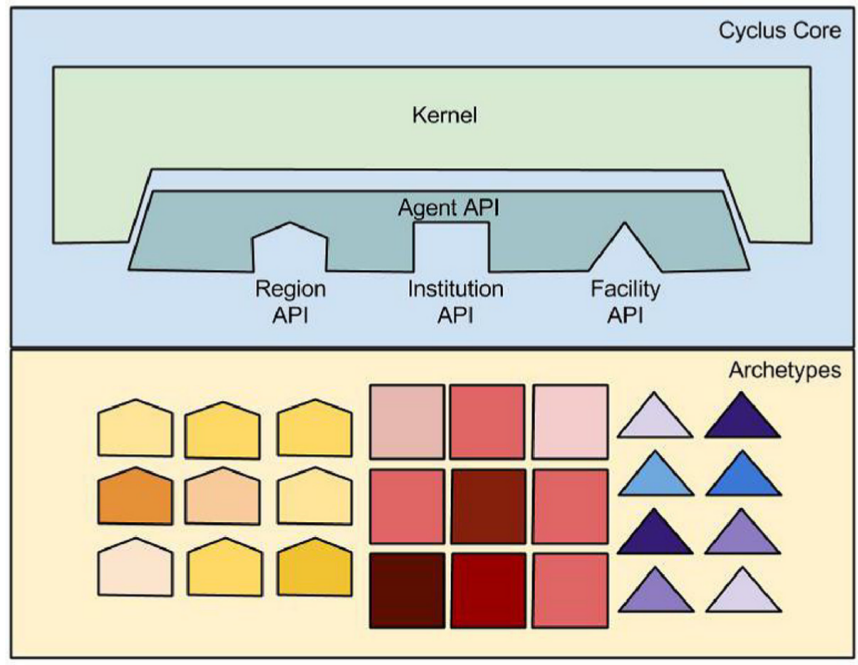
\includegraphics[width=\textwidth]{cyclus_core.png}
    \end{center}
    \caption{The \Cyclus core provides APIs that the archetypes
            can be loaded into the simulation modularly
            \cite{huff_fundamental_2016}.}
    \label{fig:core}
\end{figure}

Due to this modularity in the \Cyclus framework, the developed
model in this work can be implemented independently without
having to modify the \Cyclus source code. The new facility archetype
is simply written with the \Cyclus API, and imported in a
\Cyclus simulation.

\subsubsection{\Cycamore Recipe Reactor}
\Cycamore is a library that consists of useful
fuel cycle facility archetypes for \Cyclus. The
recipe reactor in \Cycamore is a batch-wise reactor.
A reactor core is consisted of multiple batches,
and a batch is consisted of multiple assemblies.
At startup, the reactor requests the entire core,
which is consisted of user-defined number of assemblies.
At every cycle, the reactor discharges and
requests batches of fuel. Upon decommissioning,
the reactor discharges all its fuel. The discharged
fuel is transmutated to the user-defined recipe.
No depletion calculation is performed. However,
the user can define multiple recipes, and can define
times to change the recipe from one to another.


\bibliography{bibliography}


\end{document}
